% !TeX program = xelatex
\documentclass[a4paper,10pt]{article}

% ============================================================================
% កញ្ចប់បណ្ណាល័យ (Packages) – តាមលំនាំស្តង់ដារ អនុវិទ្យាល័យព្រះក្រសាំង (ls_plan.tex)
% បរិបទ៖ ថ្នាក់រៀនគ្មានស្លាយ LCD – បង្រៀនដោយប្រើក្ដារខៀន និងសន្លឹកកិច្ចការសិស្សស-ខ្មៅជាគោល
% ============================================================================
\usepackage[a4paper, left=0.95cm, right=0.95cm, top=0.85cm, bottom=0.92cm, footskip=0.52cm]{geometry}
\usepackage{amsmath}
\usepackage{unicode-math}
\usepackage{fontspec}
\usepackage{array, longtable, multirow, colortbl}
\usepackage[table]{xcolor}
\usepackage{enumitem}
\usepackage{pifont}
\usepackage{fancyhdr}
\usepackage{tikz}
\usetikzlibrary{calc, arrows.meta, angles, quotes, decorations.markings, positioning, babel}

% LaTeX + longtable compatibility guard
\makeatletter
\let\@expl@@@mark@update@singlecol@structures@@\relax
\makeatother

% ============================================================================
% ការកំណត់ពុម្ពអក្សរផ្លូវការ (Cross-Platform Fonts Configuration)
% ============================================================================
\providecommand{\NGSFindFonts}{%
  \IfFileExists{C:/Windows/Fonts/cambria.ttc}{%
    \def\NGSSysPath{C:/Windows/Fonts/}%
    \def\NGSUserPath{C:/Users/KIT/AppData/Local/Microsoft/Windows/Fonts/}%
  }{%
    \IfFileExists{./fonts/KhmerOSsiemreap.ttf}{\def\NGSSysPath{./fonts/}\def\NGSUserPath{./fonts/}}{%
    \IfFileExists{../fonts/KhmerOSsiemreap.ttf}{\def\NGSSysPath{../fonts/}\def\NGSUserPath{../fonts/}}{%
    \IfFileExists{../../fonts/KhmerOSsiemreap.ttf}{\def\NGSSysPath{../../fonts/}\def\NGSUserPath{../../fonts/}}{%
    \IfFileExists{../../../fonts/KhmerOSsiemreap.ttf}{\def\NGSSysPath{../../../fonts/}\def\NGSUserPath{../../../fonts/}}{%
    \IfFileExists{../../../../fonts/KhmerOSsiemreap.ttf}{\def\NGSSysPath{../../../../fonts/}\def\NGSUserPath{../../../../fonts/}}{%
    \IfFileExists{../../../../../fonts/KhmerOSsiemreap.ttf}{\def\NGSSysPath{../../../../../fonts/}\def\NGSUserPath{../../../../../fonts/}}{%
    \IfFileExists{../../../../../../fonts/KhmerOSsiemreap.ttf}{\def\NGSSysPath{../../../../../../fonts/}\def\NGSUserPath{../../../../../../fonts/}}{%
      \def\NGSSysPath{../../../../../../../fonts/}\def\NGSUserPath{../../../../../../../fonts/}%
    }}}}}}}%
  }%
}
\NGSFindFonts

\setmathfont[
  Path={\NGSSysPath},
  FontIndex=1,
  Scale=1.02
]{cambria.ttc}

\defaultfontfeatures{Ligatures=TeX}

\setmainfont[
  Path={\NGSUserPath},
  Extension=.ttf,
  Script=Khmer,
  BoldFont={KhmerOSsiemreap},
  BoldFeatures={FakeBold=1.8},
  ItalicFont={KhmerOSsiemreap},
  ItalicFeatures={FakeSlant=0.25},
  BoldItalicFont={KhmerOSsiemreap},
  BoldItalicFeatures={FakeBold=1.8, FakeSlant=0.25}
]{KhmerOSsiemreap}

\newfontfamily\muol[
  Path={\NGSUserPath},
  Extension=.ttf,
  Script=Khmer
]{KhmerOSmuollight}

\newfontfamily\TimesEn[
  Path={\NGSSysPath},
  Extension=.ttf,
  Scale=1.00,
  BoldFont={timesbd},
  ItalicFont={timesi},
  BoldItalicFont={timesbi}
]{times}

\newfontfamily\NagaBold[
  Path={\NGSUserPath},
  Extension=.ttf
]{AKbalthom Naga Bold}

\newfontfamily\CalibriFont[
  Path={\NGSSysPath},
  Extension=.ttf
]{calibri}

\newfontfamily\Tacteing[
  Path={\NGSUserPath}
]{TACTENG.TTF}

\newfontfamily\CourierBullet[
  Path={\NGSSysPath},
  Extension=.ttf
]{cour}
\newcommand{\wcirc}{{\CourierBullet\fontsize{9.5pt}{11pt}\selectfont o}}

\XeTeXlinebreaklocale "km"
\XeTeXlinebreakskip = 0pt plus 1pt minus 0.1pt

% ============================================================================
% ការកំណត់ពណ៌ និងទម្រង់ទំព័រ (Colors & Page Style)
% ============================================================================
\definecolor{stepgray}{HTML}{D9D9D9}
\definecolor{headgray}{HTML}{F2F2F2}
\definecolor{boxgray}{HTML}{D9D9D9}
\definecolor{darkred}{HTML}{C00000}
\definecolor{red5e}{HTML}{FF0000}

\pagestyle{fancy}
\fancyhf{}
\renewcommand{\headrulewidth}{0pt}
\fancyfoot[R]{\CalibriFont\fontsize{11pt}{13pt}\selectfont\thepage}

\setlength{\parindent}{0pt}
\setlength{\parskip}{0pt}
\setlength{\tabcolsep}{3.8pt}

\newcolumntype{L}[1]{>{\raggedright\arraybackslash}p{#1}}

% ============================================================================
% ម៉ាក្រូជំនួយ (Helper Macros)
% ============================================================================
\newcommand{\en}[1]{{\TimesEn #1}}
\newcommand{\enbf}[1]{{\TimesEn\textbf{#1}}}
\newcommand{\unit}[1]{\,\text{\en{#1}}}
\newcommand{\fiveE}[1]{{\NagaBold\fontsize{9.5pt}{13pt}\selectfont\textcolor{red5e}{#1}}}
\newcommand{\timenote}[1]{\textcolor{darkred}{\textit{#1}}}
\newcommand{\redsub}[1]{\textcolor{darkred}{#1}}
\newcommand{\graybox}[1]{\colorbox{boxgray}{\strut\hspace{2pt}#1\hspace{2pt}}}
\newcommand{\ditem}{\tikz[baseline=-0.5ex]\fill (0,0.42ex) -- (0.42ex,0) -- (0,-0.42ex) -- (-0.42ex,0) -- cycle;\hspace{0.3em}}
\newcommand{\cnum}[1]{{\fontsize{10.5pt}{12pt}\selectfont\ding{\numexpr171+#1\relax}}\hspace{0.2em}}
\newcommand{\cfig}[1]{\par\vspace{4pt}{\centering #1\par}\vspace{4pt}}
\newcommand{\stepheader}[1]{\multicolumn{3}{|c|}{\cellcolor{stepgray}\muol #1} \\* \noalign{\hrule height 0.4pt}}
\newcommand{\tri}[1]{\ensuremath{\triangle #1}}
\newcommand{\ang}[1]{\ensuremath{\angle #1}}
\newcommand{\cg}{\ensuremath{\cong}}
\newcommand{\khmflourish}{{\Tacteing\fontsize{36pt}{14pt}\selectfont\raisebox{-5pt}{3}}}

% រចនាប័ទ្មសញ្ញាសម្គាល់ស-ខ្មៅ (Monochrome Symbolic Coding)
\tikzset{
  tk1/.style={postaction={decorate},decoration={markings,mark=at position 0.50 with {\draw[black, line width=0.85pt](0,-0.095)--(0,0.095);}}},
  tk2/.style={postaction={decorate},decoration={markings,
    mark=at position 0.45 with {\draw[black, line width=0.85pt](0,-0.095)--(0,0.095);},
    mark=at position 0.55 with {\draw[black, line width=0.85pt](0,-0.095)--(0,0.095);}}},
  par1/.style={postaction={decorate},decoration={markings,mark=at position 0.52 with {\draw[black, line width=0.85pt](-0.07,0.08)--(0.05,0)--(-0.07,-0.08);}}},
  par2/.style={postaction={decorate},decoration={markings,
    mark=at position 0.46 with {\draw[black, line width=0.85pt](-0.07,0.08)--(0.05,0)--(-0.07,-0.08);},
    mark=at position 0.58 with {\draw[black, line width=0.85pt](-0.07,0.08)--(0.05,0)--(-0.07,-0.08);}}}
}

\newcommand{\rightbox}[4][0.20]{%
  \draw[black, line width=0.8pt]
    ($(#3)!#1!(#2)$) -- ($($(#3)!#1!(#2)$)+($(#3)!#1!(#4)$)-(#3)$) -- ($(#3)!#1!(#4)$);
}

% ============================================================================
% ម៉ាក្រូរូបភាពធរណីមាត្រស-ខ្មៅ (Proportional 3.8–7.2 cm B&W TikZ Diagrams)
% ============================================================================

% ១. រំលឹកមេរៀនទាក់ទង៖ បន្ទាត់ស្រប (ដែកកែងរអិល) និងផលបូកមុំក្នុងចតុកោណ 360°
\newcommand{\figPrereqQUAD}{%
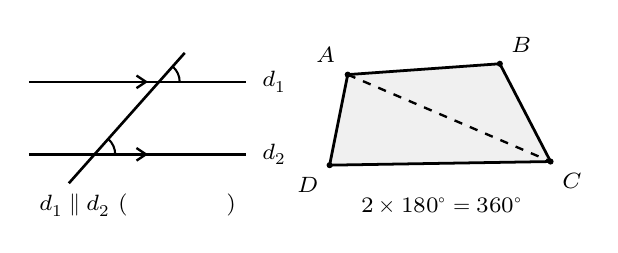
\begin{tikzpicture}[scale=0.92, every node/.style={font=\footnotesize, text=black}]
  % ឆ្វេង៖ បន្ទាត់ស្របដោយមុំត្រូវគ្នា / ដែកកែង
  \begin{scope}[shift={(0,0)}]
    \draw[black, line width=0.95pt, par1] (0,1.25) -- (3.0,1.25) node[right=2pt] {$d_1$};
    \draw[black, line width=0.95pt, par1] (0,0.25) -- (3.0,0.25) node[right=2pt] {$d_2$};
    \draw[black, line width=0.95pt] (0.55,-0.15) -- (2.15,1.65);
    \draw[black, line width=0.75pt] ($(0.91,0.25)+(0:0.28)$) arc (0:48:0.28);
    \draw[black, line width=0.75pt] ($(1.80,1.25)+(0:0.28)$) arc (0:48:0.28);
    \node at (1.50,-0.45) {$d_1 \parallel d_2$ (មុំត្រូវគ្នាស្មើ)};
  \end{scope}
  % ស្ដាំ៖ ចតុកោណបំបែកជា ២ ត្រីកោណ => 360°
  \begin{scope}[shift={(4.15,0)}]
    \coordinate (A) at (0.25,1.35);
    \coordinate (B) at (2.35,1.50);
    \coordinate (C) at (3.05,0.15);
    \coordinate (D) at (0,0.10);
    \fill[gray!12] (A)--(B)--(C)--(D)--cycle;
    \draw[black, line width=1.0pt] (A)--(B)--(C)--(D)--cycle;
    \draw[black, line width=0.85pt, dashed] (A)--(C);
    \fill[black] (A) circle (1.2pt) node[above left=1pt] {$A$};
    \fill[black] (B) circle (1.2pt) node[above right=1pt] {$B$};
    \fill[black] (C) circle (1.2pt) node[below right=1pt] {$C$};
    \fill[black] (D) circle (1.2pt) node[below left=1pt] {$D$};
    \node at (1.55,-0.45) {$2 \times 180^\circ = 360^\circ$};
  \end{scope}
\end{tikzpicture}}

% ២. E1 Engage: ក្បឿងដាក់ត្រង់ vs ក្បឿងដាក់បង្វិល 45° (Prototype Bias Hook)
\newcommand{\figEngageQUAD}{%
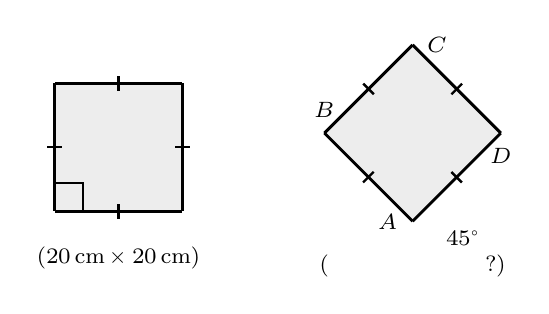
\begin{tikzpicture}[scale=0.90, every node/.style={font=\footnotesize, text=black}]
  % ក្បឿងទី១៖ ដាក់ត្រង់
  \begin{scope}[shift={(0,0.18)}]
    \coordinate (A) at (0,0);
    \coordinate (B) at (1.80,0);
    \coordinate (C) at (1.80,1.80);
    \coordinate (D) at (0,1.80);
    \fill[gray!14] (A)--(B)--(C)--(D)--cycle;
    \draw[black, line width=1.05pt, tk1] (A)--(B);
    \draw[black, line width=1.05pt, tk1] (B)--(C);
    \draw[black, line width=1.05pt, tk1] (C)--(D);
    \draw[black, line width=1.05pt, tk1] (D)--(A);
    \rightbox[0.22]{B}{A}{D}
  \end{scope}
  \node[align=center] at (0.90,-0.42) {ក្បឿងដាក់ត្រង់\\($20\unit{cm}\times 20\unit{cm}$)};
  % ក្បឿងទី២៖ ក្បឿងដដែលបង្វិល 45°
  \begin{scope}[shift={(5.05,1.28)}, rotate=45]
    \coordinate (P) at (-0.88,-0.88);
    \coordinate (Q) at (0.88,-0.88);
    \coordinate (R) at (0.88,0.88);
    \coordinate (S) at (-0.88,0.88);
    \fill[gray!14] (P)--(Q)--(R)--(S)--cycle;
    \draw[black, line width=1.05pt, tk1] (P)--(Q);
    \draw[black, line width=1.05pt, tk1] (Q)--(R);
    \draw[black, line width=1.05pt, tk1] (R)--(S);
    \draw[black, line width=1.05pt, tk1] (S)--(P);
    \node[above=2pt] at (S) {$B$};
    \node[right=2pt] at (R) {$C$};
    \node[below=2pt] at (Q) {$D$};
    \node[left=2pt] at (P) {$A$};
  \end{scope}
  \node[align=center] at (5.05,-0.42) {ក្បឿងដដែលបង្វិល $45^\circ$\\(តើនៅជាការេ និងចតុកោណកែងទេ?)};
\end{tikzpicture}}

% ៣. E2 Explore: ប្រភេទចតុកោណគោលទាំង ៥ តាមសៀវភៅគោល ទំ.១៦៩–១៧០
\newcommand{\figFiveTypesQUAD}{%
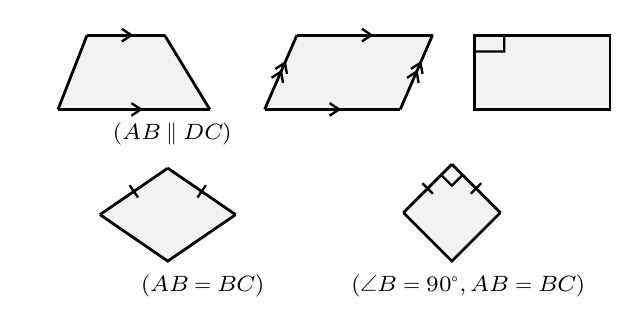
\begin{tikzpicture}[scale=0.82, every node/.style={font=\footnotesize, text=black}]
  % 1. ចតុកោណព្នាយ
  \begin{scope}[shift={(0,2.35)}]
    \coordinate (D) at (0,0); \coordinate (C) at (2.35,0);
    \coordinate (B) at (1.65,1.15); \coordinate (A) at (0.45,1.15);
    \fill[gray!10] (A)--(B)--(C)--(D)--cycle;
    \draw[black, line width=1.0pt, par1] (A)--(B);
    \draw[black, line width=1.0pt, par1] (D)--(C);
    \draw[black, line width=1.0pt] (D)--(A) (C)--(B);
    \node at (1.18,-0.38) {ចតុកោណព្នាយ ($AB\parallel DC$)};
  \end{scope}
  % 2. ប្រលេឡូក្រាម
  \begin{scope}[shift={(3.20,2.35)}]
    \coordinate (D) at (0,0); \coordinate (C) at (2.10,0);
    \coordinate (B) at (2.60,1.15); \coordinate (A) at (0.50,1.15);
    \fill[gray!10] (A)--(B)--(C)--(D)--cycle;
    \draw[black, line width=1.0pt, par1] (A)--(B);
    \draw[black, line width=1.0pt, par1] (D)--(C);
    \draw[black, line width=1.0pt, par2] (D)--(A);
    \draw[black, line width=1.0pt, par2] (C)--(B);
    \node at (1.30,-0.38) {ប្រលេឡូក្រាម};
  \end{scope}
  % 3. ចតុកោណកែង
  \begin{scope}[shift={(6.45,2.35)}]
    \coordinate (D) at (0,0); \coordinate (C) at (2.10,0);
    \coordinate (B) at (2.10,1.15); \coordinate (A) at (0,1.15);
    \fill[gray!10] (A)--(B)--(C)--(D)--cycle;
    \draw[black, line width=1.0pt] (A)--(B)--(C)--(D)--cycle;
    \rightbox[0.22]{D}{A}{B}
    \node at (1.05,-0.38) {ចតុកោណកែង};
  \end{scope}
  % 4. ចតុកោណស្មើ
  \begin{scope}[shift={(0.65,0)}]
    \coordinate (A) at (0,0.72); \coordinate (B) at (1.05,1.44);
    \coordinate (C) at (2.10,0.72); \coordinate (D) at (1.05,0);
    \fill[gray!10] (A)--(B)--(C)--(D)--cycle;
    \draw[black, line width=1.0pt, tk1] (A)--(B);
    \draw[black, line width=1.0pt, tk1] (B)--(C);
    \draw[black, line width=1.0pt] (C)--(D)--(A);
    \node at (1.05,-0.38) {ចតុកោណស្មើ ($AB=BC$)};
  \end{scope}
  % 5. ការេ (បង្វិល 45° តាមសៀវភៅគោល ទំ.១៧០)
  \begin{scope}[shift={(5.35,0)}]
    \coordinate (A) at (0,0.75); \coordinate (B) at (0.75,1.50);
    \coordinate (C) at (1.50,0.75); \coordinate (D) at (0.75,0);
    \fill[gray!10] (A)--(B)--(C)--(D)--cycle;
    \draw[black, line width=1.0pt, tk1] (A)--(B);
    \draw[black, line width=1.0pt, tk1] (B)--(C);
    \draw[black, line width=1.0pt] (C)--(D)--(A);
    \rightbox[0.22]{A}{B}{C}
    \node at (0.75,-0.38) {ការេ ($\ang{B}=90^\circ, AB=BC$)};
  \end{scope}
\end{tikzpicture}}

% ៤. E3 Explain: គំនូសតាងទំនាក់ទំនងនៃប្រភេទចតុកោណ (តាមសៀវភៅគោល ទំ.១៧០ បេះបិទ)
\newcommand{\figHierarchyQUAD}{%
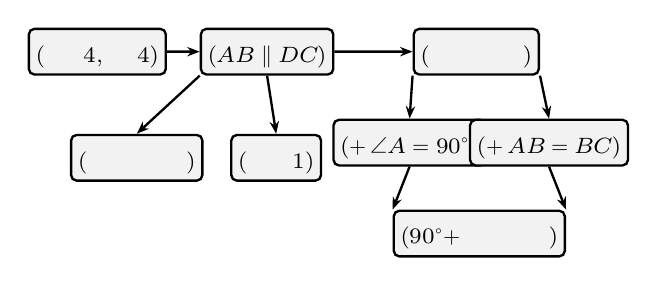
\begin{tikzpicture}[scale=0.77, every node/.style={font=\footnotesize, text=black},
  box/.style={draw=black, line width=0.85pt, rounded corners=2pt, fill=gray!10, inner sep=2.5pt, align=center}]
  \node[box] (quad) at (0,2.35) {\textbf{ចតុកោណ}\\(ជ្រុង $4$, មុំ $4$)};
  \node[box] (trap) at (2.80,2.35) {\textbf{ចតុកោណព្នាយ}\\($AB\parallel DC$)};
  \node[box] (para) at (6.25,2.35) {\textbf{ប្រលេឡូក្រាម}\\(ជ្រុងឈមស្របពីរៗ)};

  \node[box] (isotrap) at (0.65,0.60) {ព្នាយសមបាទ\\(ជ្រុងមិនស្របស្មើ)};
  \node[box] (rttrap)  at (2.95,0.60) {ព្នាយកែង\\(មុំកែង $1$)};

  \node[box] (rect) at (5.15,0.85) {\textbf{ចតុកោណកែង}\\($+\,\ang{A}=90^\circ$)};
  \node[box] (rhom) at (7.45,0.85) {\textbf{ចតុកោណស្មើ}\\($+\,AB=BC$)};
  \node[box] (sq)   at (6.30,-0.65) {\textbf{ការេ}\\($90^\circ +$ ជ្រុងជាប់ស្មើ)};

  \draw[-{Stealth[length=4.5pt]}, line width=0.85pt] (quad) -- (trap);
  \draw[-{Stealth[length=4.5pt]}, line width=0.85pt] (trap) -- (para);
  \draw[-{Stealth[length=4.5pt]}, line width=0.85pt] (trap.south west) -- (isotrap.north);
  \draw[-{Stealth[length=4.5pt]}, line width=0.85pt] (trap.south) -- (rttrap.north);
  \draw[-{Stealth[length=4.5pt]}, line width=0.85pt] (para.south west) -- (rect.north);
  \draw[-{Stealth[length=4.5pt]}, line width=0.85pt] (para.south east) -- (rhom.north);
  \draw[-{Stealth[length=4.5pt]}, line width=0.85pt] (rect.south) -- (sq.north west);
  \draw[-{Stealth[length=4.5pt]}, line width=0.85pt] (rhom.south) -- (sq.north east);
\end{tikzpicture}}

% ៥. E4 Elaborate: រូបភាពលំហាត់គំរូ ៤ ករណី (រួមទាំងអន្ទាក់ព្នាយសមបាទ និងរូបបង្វិល)
\newcommand{\figModelQUAD}{%
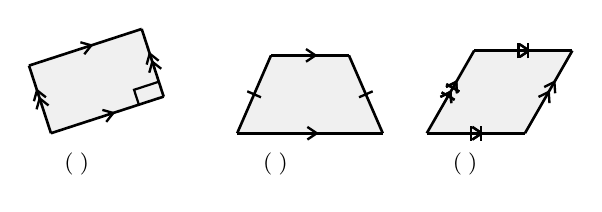
\begin{tikzpicture}[scale=0.86, every node/.style={font=\footnotesize, text=black}]
  % (ក) ចតុកោណកែងបង្វិល 20°
  \begin{scope}[shift={(0,0)}, rotate=18]
    \coordinate (A) at (0,0); \coordinate (B) at (1.75,0);
    \coordinate (C) at (1.75,1.05); \coordinate (D) at (0,1.05);
    \fill[gray!12] (A)--(B)--(C)--(D)--cycle;
    \draw[black, line width=0.95pt, par1] (D)--(C);
    \draw[black, line width=0.95pt, par1] (A)--(B);
    \draw[black, line width=0.95pt, par2] (A)--(D);
    \draw[black, line width=0.95pt, par2] (B)--(C);
    \rightbox[0.22]{A}{B}{C}
  \end{scope}
  \node at (0.85,-0.45) {(ក) ចតុកោណកែង};

  % (ខ) ព្នាយសមបាទ (អន្ទាក់ MN||PO តែ MP=NO)
  \begin{scope}[shift={(2.75,0)}]
    \coordinate (P) at (0,0); \coordinate (O) at (2.15,0);
    \coordinate (N) at (1.65,1.15); \coordinate (M) at (0.50,1.15);
    \fill[gray!12] (M)--(N)--(O)--(P)--cycle;
    \draw[black, line width=0.95pt, par1] (M)--(N);
    \draw[black, line width=0.95pt, par1] (P)--(O);
    \draw[black, line width=0.95pt, tk1] (P)--(M);
    \draw[black, line width=0.95pt, tk1] (O)--(N);
    \node at (1.08,-0.45) {(ខ) ព្នាយសមបាទ};
  \end{scope}

  % (គ) ចតុកោណស្មើទ្រេត
  \begin{scope}[shift={(5.55,0)}]
    \coordinate (E) at (0,0); \coordinate (F) at (1.45,0);
    \coordinate (G) at (2.15,1.22); \coordinate (H) at (0.70,1.22);
    \fill[gray!12] (E)--(F)--(G)--(H)--cycle;
    \draw[black, line width=0.95pt, par1, tk2] (H)--(G);
    \draw[black, line width=0.95pt, par1, tk2] (E)--(F);
    \draw[black, line width=0.95pt, par2, tk2] (E)--(H);
    \draw[black, line width=0.95pt, par2] (F)--(G);
    \node at (1.08,-0.45) {(គ) ចតុកោណស្មើ};
  \end{scope}
\end{tikzpicture}}

% ============================================================================
% ចាប់ផ្ដើមឯកសារ (Document Body)
% ============================================================================
\begin{document}
\fontsize{10pt}{15.2pt}\selectfont

% -------------------- ក្បាលកិច្ចតែងការ (Header) --------------------
\begin{center}
  {\muol\fontsize{11pt}{16pt}\selectfont ព្រះរាជាណាចក្រកម្ពុជា}\\[2pt]
  {\muol\fontsize{10pt}{15pt}\selectfont ជាតិ សាសនា ព្រះមហាក្សត្រ}\\[1pt]
  \khmflourish
\end{center}

\vspace{-28pt}
{\muol\fontsize{9.5pt}{12.5pt}\selectfont
មន្ទីរអប់រំ យុវជន និងកីឡា ខេត្តកំពង់ធំ\\
ការិយាល័យអប់រំ យុវជន និងកីឡា ស្រុកកំពង់ស្វាយ\\
អនុវិទ្យាល័យព្រះក្រសាំង}

\vspace{1pt}
\begin{center}
  {\muol\fontsize{10pt}{14pt}\selectfont កិច្ចតែងការបង្រៀន}
\end{center}
\vspace{0pt}

% -------------------- ព័ត៌មានទូទៅ (Metadata) --------------------
{\renewcommand{\arraystretch}{0.95}
\hspace*{4.05cm}%
\begin{tabular}{@{}l l l@{}}
  - \hspace{0.35cm} មុខវិជ្ជា & : & គណិតវិទ្យា ថ្នាក់ទី៨ \\
  - \hspace{0.35cm} ចំណងជើងមេរៀន & : & មេរៀនទី១៣ ចតុកោណ \\
  - \hspace{0.35cm} ចំណងជើងរង & : & ១. ប្រភេទនៃចតុកោណ (ទំព័រ ១៦៩--១៧០) \\
  - \hspace{0.35cm} រយៈពេល & : & ១ ម៉ោងសិក្សា (៥០ នាទី) \\
  - \hspace{0.35cm} បង្រៀនដោយ & : & ហុក ប៊ុនថែន \\
  - \hspace{0.35cm} កាលបរិច្ឆេទ & : & ថ្ងៃសុក្រ ២កើត ខែមិគសិរ ព.ស.២៥៧០ (១១ ធ្នូ ២០២៦) \\
\end{tabular}

\vspace{1pt}

% -------------------- I. វត្ថុបំណង --------------------
\textbf{I.} {\muol វត្ថុបំណង}\\[1pt]
\hspace*{0.55cm}%
\begin{tabular}{@{}l l L{14.2cm}@{}}
  \wcirc \hspace{0.25cm} វិជ្ជាសម្បទា & : & សិស្សប្រាប់និយមន័យត្រឹមត្រូវនៃប្រភេទចតុកោណទាំងអស់ (ចតុកោណ ចតុកោណព្នាយ ព្នាយសមបាទ ព្នាយកែង ប្រលេឡូក្រាម ចតុកោណកែង ចតុកោណស្មើ និងការេ) និងពន្យល់គំនូសតាងទំនាក់ទំនងនៃប្រភេទចតុកោណតាមសៀវភៅគោល (ទំ.១៦៩--១៧០, កែពាក្យខុស «ចតុកោណកោណកែង» ទៅ «ចតុកោណកែង») ។ \\
  \wcirc \hspace{0.25cm} បំណិនសម្បទា & : & សិស្សប្រើបន្ទាត់ក្រិត និងដែកកែងវាស់ពិនិត្យភាពស្រប ជ្រុងប៉ុនគ្នា និងមុំកែងលើសន្លឹកកិច្ចការស-ខ្មៅ បំពេញតារាងវិភាគលក្ខណៈ \en{Van Hiele} សង់មែកធាងឋានានុក្រមចតុកោណ និងបកស្រាយសំណើពិត-មិនពិតលើរូបបង្វិល $45^\circ$ ដោយប្រើសញ្ញាសម្គាល់ \textbf{[tracing]} និងធនាគារនិយមន័យ \cnum{1}--\cnum{5} ។ \\
  \wcirc \hspace{0.25cm} ចរិយាសម្បទា & : & សិស្សមានទម្លាប់ពិនិត្យលក្ខខណ្ឌគណិតវិទ្យាជំនួសការស្មានតាមរាងទម្លាប់ភ្នែក (\en{Prototype Bias}) ចូលរួមពិភាក្សាជាដៃគូលើសន្លឹកកិច្ចការយ៉ាងសកម្ម និងផ្សារភ្ជាប់ទម្រង់ចតុកោណទៅនឹងសំណង់ក្បឿង និងស៊ុមបង្អួចក្នុងជីវភាពពិត ។ \\
\end{tabular}

\vspace{1pt}

% -------------------- II. សម្ភារៈឧបទេស --------------------
\textbf{II.} {\muol សម្ភារៈឧបទេស}\\[1pt]
\hspace*{0.55cm}$\bullet$ \hspace{0.35cm} សៀវភៅសិក្សាគោលគណិតវិទ្យាថ្នាក់ទី៨ (ទំ.១៦៩--១៧០ និងទំ.១៨៥) ក្ដារខៀន ដីស បន្ទាត់ក្រិត ដែកកែង រ៉ាប់ព័រទ័រ និងសន្លឹកកិច្ចការសិស្សស-ខ្មៅ (\en{Worksheet\_QUAD1} ចំនួន ២ ទំព័រ \en{A4} សម្រាប់បំពេញផ្ទាល់ ដោយមិនប្រើស្លាយ \en{LCD} ឬកន្ត្រៃកាត់) ។

\vspace{1pt}

% -------------------- III. វិធីសាស្រ្តបង្រៀន --------------------
\textbf{III.} {\muol វិធីសាស្រ្តបង្រៀន}\\[1pt]
\hspace*{0.45cm}%
\begin{tabular}{@{}l l L{14.85cm}@{}}
  $\bullet$ \hspace{0.25cm} គោលវិធី & : & សិស្សមជ្ឈមណ្ឌល (សិក្សាស៊ើបអង្កេតជាដៃគូលើសន្លឹកកិច្ចការបំពេញផ្ទាល់ គ្មានស្លាយ \en{LCD}) \\
  $\bullet$ \hspace{0.25cm} យុទ្ធវិធីបង្រៀន & : & គម្រូស្ថាបនានិយម \en{5Es} រួមបញ្ចូល \textbf{តារាងវិភាគលក្ខណៈ \en{Van Hiele} និងមែកធាងឋានានុក្រមរួមបញ្ចូល} (\en{De Villiers, 1994; Fujita, 2012} — បំបែកអន្ទាក់រាងគំរូ \en{Prototype Bias} តាម \en{POE}, \textbf{[tracing]} និង \cnum{1}--\cnum{5}) \\
\end{tabular}
}

\vspace{1pt}

% -------------------- IV. ដំណើរការបង្រៀន --------------------
\textbf{IV.} {\muol ដំណើរការបង្រៀន}

\vspace{1pt}

% ============================================================================
% តារាងដំណើរការបង្រៀន (Granular Multi-Row 3-Column Table – 50 នាទី)
% ============================================================================
\renewcommand{\arraystretch}{1.15}
\begin{longtable}{|L{5.50cm}|L{7.90cm}|L{4.80cm}|}
\hline
\rowcolor{headgray}
\multicolumn{1}{|c|}{\muol សកម្មភាពគ្រូ} &
\multicolumn{1}{c|}{\muol ខ្លឹមសារមេរៀន} &
\multicolumn{1}{c|}{\muol សកម្មភាពសិស្ស} \\
\hline
\endfirsthead

\hline
\endhead

\hline
\endfoot

\hline
\endlastfoot

% ==================== ជំហានទី១ (2min) ====================
\stepheader{ជំហានទី១ \enbf{(}រដ្ឋបាលថ្នាក់\enbf{)}}
$\bullet$ ពិនិត្យអវត្តមាន សណ្ដាប់ធ្នាប់ អនាម័យ និងសម្ភារៈសិក្សា (បន្ទាត់ក្រិត ដែកកែង រ៉ាប់ព័រទ័រ)
&
$\bullet$ ពិនិត្យវត្តមាន និងសណ្ដាប់ធ្នាប់ថ្នាក់រៀន \par
$\bullet$ ត្រៀមបន្ទាត់ក្រិត និងដែកកែងសម្រាប់វាស់លើសន្លឹកកិច្ចការ
&
$\circ$ ប្រធានថ្នាក់រាយការណ៍អវត្តមាន និងត្រៀមឧបករណ៍ធរណីមាត្រ \\[3pt]

$\bullet$ រៀបចំសិស្សជាដៃគូពិភាក្សា («ក្រុមអ្នកត្រួតពិនិត្យពុម្ពក្បឿង និងស៊ុមបង្អួច») រួចចែកសន្លឹកកិច្ចការ \en{Worksheet\_QUAD1} ផ្កាប់លើតុ
&
$\bullet$ ការចាត់ដៃគូសិក្សា និងចែកសន្លឹកកិច្ចការស-ខ្មៅ (២ ទំព័រ \en{A4})
&
$\circ$ អង្គុយតាមដៃគូ និងទទួលសន្លឹកកិច្ចការទុកលើតុ \\
\hline

% ==================== ជំហានទី២ (9min: <=3 + 3 + E1 3) ====================
\stepheader{ជំហានទី២ \enbf{(}កិច្ចការផ្ទះ \enbf{+} ទំនាក់ទំនងមេរៀនថ្មី\enbf{)}}
\ditem \textbf{កំណែកិច្ចការផ្ទះ ($\le 3\unit{min}$)} \timenote{សង្ខេបខ្លីលើក្ដារខៀន}
&
{\centering\redsub{កំណែកិច្ចការផ្ទះមេរៀនទី១២ និងចំណុចគន្លឹះ}\par}
&
$\circ$ យកសៀវភៅកិច្ចការផ្ទះមកផ្ទៀងផ្ទាត់ \\[2pt]

$\bullet$ ផ្ទៀងលំហាត់សំយោគចុងមេរៀនទី១២ និងរំលឹកលក្ខខណ្ឌមុំឆ្លាស់ក្នុងនៃបន្ទាត់ស្រប
&
$\bullet$ បើបន្ទាត់ពីរកាត់ដោយបន្ទាត់កាត់មួយបង្កើតមុំឆ្លាស់ក្នុងស្មើគ្នា ឬមុំត្រូវគ្នាស្មើគ្នា នោះបន្ទាត់ទាំងពីរ\textbf{ស្របគ្នា} ($d_1 \parallel d_2$) ។
&
$\circ$ កែចំណុចខ្វះខាតក្នុងសៀវភៅកិច្ចការផ្ទះ \\[3pt]

\ditem \textbf{រំលឹកមេរៀនទាក់ទង ($3\unit{min}$)} \par
$\bullet$ គូសរូបលើក្ដារខៀន សួររំលឹក៖ \par
– \textbf{សំណួរទី១៖} តើគេប្រើដែកកែង និងបន្ទាត់ក្រិតពិនិត្យថា $d_1 \parallel d_2$ ដូចម្ដេច? \par
– \textbf{សំណួរទី២៖} បើគូសអង្កត់ទ្រូង $AC$ ១ ខ្សែ តើផលបូកមុំក្នុងចតុកោណ $ABCD$ ស្មើប៉ុន្មានដឺក្រេ?
&
{\centering\redsub{រំលឹកមេរៀនទាក់ទងមេរៀនថ្មី}\par} \par
$\bullet$ \textbf{ពិនិត្យភាពស្រប៖} រអិលដែកកែងតាមបន្ទាត់បន្ទាល់ បើគែមកែងជួបបន្ទាត់ទាំងពីរពេញទំហឹង នោះ $d_1 \parallel d_2$ ។ \par
$\bullet$ \textbf{ផលបូកមុំក្នុងចតុកោណ៖} អង្កត់ទ្រូង $AC$ ចែក $ABCD$ ជា ២ ត្រីកោណ $\Rightarrow 2 \times 180^\circ = 360^\circ$ ។
&
$\circ$ សង្កេតរូបលើក្ដារខៀន និងឆ្លើយ៖ \par
«រអិលដែកកែងតាមបន្ទាត់បន្ទាល់ ហើយផលបូកមុំក្នុងចតុកោណស្មើ $360^\circ$» \\[3pt]

&
\cfig{\figPrereqQUAD}
& \\[3pt]

\fiveE{E1 - Engage (3min)} \timenote{(កុំទាន់ផ្ដល់ចម្លើយ)} \par
\ditem \textbf{បញ្ហាភ្ញាក់ផ្អើល «ក្បឿងការេដាក់បង្វិល $45^\circ$»៖} \par
$\bullet$ គូសក្បឿងការេ $20\unit{cm}\times 20\unit{cm}$ ចំនួន ២ ទីតាំងលើក្ដារខៀន (ដាក់ត្រង់ និងបង្វិល $45^\circ$)
&
{\centering\redsub{ស្ថានភាពបញ្ហា៖ ជាងរៀបក្បឿងនៅកំពង់ស្វាយ}\par}
&
$\circ$ សង្កេតរូបក្បឿងទាំង ២ ទីតាំងលើក្ដារខៀន និងលើក្បាលសន្លឹកកិច្ចការ \\[3pt]

&
\cfig{\figEngageQUAD}
& \\[3pt]

– \textbf{សំណួរបំផុស៖} «ជាង ក អះអាងថាក្បឿងបង្វិល $45^\circ$ ក្លាយជាចតុកោណស្មើ លែងជាការេ ឬចតុកោណកែងហើយ! រីឯជាង ខ ថាវាជាការេ ជាចតុកោណស្មើ និងជាចតុកោណកែងក្នុងពេលតែមួយ! តើដៃគូអ្នកគាំទ្រនរណា?»
&
\textbf{ចម្ងល់គោលប្រចាំម៉ោង៖} \par
(១) តើការបង្វិលរូប $45^\circ$ ធ្វើឱ្យបាត់បង់មុំកែង ឬប្រវែងជ្រុងដែរឬទេ? \par
(២) តើរូបតែមួយអាចមានឈ្មោះចតុកោណច្រើនប្រភេទរួមគ្នាបានដោយរបៀបណា?
&
$\circ$ ពិភាក្សាជាដៃគូ ៣០ វិនាទី រួចគូសធីកការទស្សន៍ទាយដំបូងក្នុងប្រអប់ \en{E1} លើសន្លឹកកិច្ចការ \\
\hline

% ==================== ជំហានទី៣ (17min: E2 11m + E3 6m) ====================
\stepheader{ជំហានទី៣ \enbf{(}ខ្លឹមសារមេរៀនថ្មី\enbf{)}}
\fiveE{E2 - Explore (11min)} \par
$\bullet$ សរសេរចំណងជើងមេរៀនទី១៣ និងចំណងជើងរងលើក្ដារខៀន (កែពាក្យបោះពុម្ពខុសក្នុងប្រអប់វត្ថុបំណងទំ.១៦៩ «ចតុកោណកោណកែង» $\to$ «ចតុកោណកែង»)
&
មេរៀនទី១៣ \hspace{0.15cm} {\muol ចតុកោណ} \par
១. ប្រភេទនៃចតុកោណ (ទំព័រ ១៦៩--១៧០)
&
$\circ$ កត់ចំណងជើងមេរៀនចូលសៀវភៅសរសេរ និងបើកសន្លឹកកិច្ចការទំព័រទី១ \\[3pt]

\ditem \textbf{សកម្មភាពទី១៖ តារាងវិភាគលក្ខណៈ \en{Van Hiele} ($6\unit{min}$)} \par
$\bullet$ ណែនាំឱ្យដៃគូសិស្សប្រើបន្ទាត់ក្រិត និងដែកកែងវាស់ពិនិត្យរូប $Q_1$--$Q_6$ លើសន្លឹកកិច្ចការ រួចដាក់សញ្ញាសម្គាល់ស-ខ្មៅ (`>`, `>>`, `|`, ប្រអប់មុំកែង) និងបំពេញតារាង
&
{\centering\textbf{ការរុករកលក្ខណៈសម្គាល់លើសន្លឹកកិច្ចការ (\en{Section 1})}\par} \par
$\bullet$ \textbf{ចតុកោណ} ជាពហុកោណដែលមានជ្រុង $4$ និងមុំ $4$ ។ \par
$\bullet$ សិស្សវាស់ពិនិត្យលក្ខខណ្ឌ ៣ គោលលើរូប $Q_1$--$Q_6$៖ \par
(១) ចំនួនគូជ្រុងឈមស្របគ្នា ($1$ គូ ឬ $2$ គូ) \par
(២) ជ្រុងជាប់គ្នាប៉ុនគ្នា ($AB=BC$) \quad (៣) មុំកែងមួយ ($\ang{A}=90^\circ$) ។
&
$\circ$ ប្រើបន្ទាត់ និងដែកកែងវាស់រូប $Q_1$--$Q_6$ គូសសញ្ញា \textbf{[tracing]} លើរូប និងបំពេញតារាងវិភាគលក្ខណៈជាដៃគូ \\[3pt]

&
\cfig{\figFiveTypesQUAD}
& \\[3pt]

\ditem \textbf{សកម្មភាពទី២៖ \en{POE} បំបែកអន្ទាក់រាងគំរូ ($5\unit{min}$)} \par
$\bullet$ \textbf{POE 2A៖} ឱ្យសិស្សយកជ្រុងកែងនៃដែកកែងដាក់ផ្ទៀងលើកំពូល $A, B, C, D$ នៃការេបង្វិល $45^\circ$ លើសន្លឹកកិច្ចការ \par
– \textbf{សំណួរ៖} តើមុំនៅកំពូលទាំង ៤ នៅតែស្មើ $90^\circ$ ឬទេ? តើវាបំពេញនិយមន័យចតុកោណកែង និងចតុកោណស្មើដែរឬទេ?
&
$\bullet$ \textbf{លទ្ធផល POE 2A (បំបែក \en{Prototype Bias})៖} \par
ការបង្វិលរូប $45^\circ$ មិនផ្លាស់ប្ដូររង្វាស់មុំ $90^\circ$ ឬប្រវែងជ្រុងឡើយ! \par
$\Rightarrow$ ការេមានជ្រុងឈមស្របពីរៗ + មុំកែងមួយ (ជា\textbf{ចតុកោណកែង}) ហើយមានជ្រុងជាប់ប៉ុនគ្នា (ជា\textbf{ចតុកោណស្មើ}) ។ \par
$\bullet$ \textbf{លទ្ធផល POE 2B (ទិសដៅព្រួញរួមបញ្ចូល)៖} \par
\graybox{គ្រប់ការេជាចតុកោណកែង \ding{51}} តែ \graybox{គ្រប់ចតុកោណកែងមិនមែនសុទ្ធតែជាការេទេ \ding{55}} (ឧ. បណ្ដោយ $4\unit{cm}\neq$ ទទឹង $2\unit{cm}$) ។
&
$\circ$ ដាក់ដែកកែងផ្ទៀងលើការេបង្វិល $45^\circ$ ឃើញមុំ $90^\circ$ ពិតប្រាកដ និងបំពេញសេចក្ដីសន្និដ្ឋាន \en{POE} លើសន្លឹកកិច្ចការ \\[3pt]

\fiveE{E3 - Explain (6min)} \par
\ditem \textbf{បង្គុំនិយមន័យផ្លូវការតាមសៀវភៅគោល (ទំ.១៦៩--១៧០)៖} \par
$\bullet$ ហៅតំណាងដៃគូឡើងបំពេញនិយមន័យទាំង ៥ និងគូសភ្ជាប់ព្រួញគំនូសតាងឋានានុក្រមលើក្ដារខៀន
&
\textbf{សង្ខេបនិយមន័យគោល និងធនាគារហេតុផល \cnum{1}--\cnum{5}៖} \par
\cnum{1} \textbf{ចតុកោណព្នាយ៖} ចតុកោណដែលមានជ្រុងពីរស្របគ្នា ($AB\parallel DC$) ។ (បើជ្រុងមិនស្របស្មើគ្នា $\to$ \textbf{ព្នាយសមបាទ}; បើមានមុំកែងមួយ $\to$ \textbf{ព្នាយកែង}) ។ \par
\cnum{2} \textbf{ប្រលេឡូក្រាម៖} ចតុកោណដែលមានជ្រុងឈមស្របគ្នាពីរៗ ($AB\parallel CD$ និង $AD\parallel BC$) ។
&
$\circ$ តំណាងដៃគូឡើងបង្ហាញលទ្ធផល និងផ្ទៀងផ្ទាត់និយមន័យ \cnum{1}--\cnum{2} ក្នុងប្រអប់សង្ខេបលើសន្លឹកកិច្ចការ \\[3pt]

$\bullet$ សង្កត់ធ្ងន់លើការបន្ថែមលក្ខខណ្ឌពីប្រលេឡូក្រាមទៅជា ចតុកោណកែង ចតុកោណស្មើ និងការេ
&
\cnum{3} \textbf{ចតុកោណកែង៖} ប្រលេឡូក្រាមដែលមានមុំកែងមួយ ($\ang{A}=90^\circ$) ។ \par
\cnum{4} \textbf{ចតុកោណស្មើ៖} ប្រលេឡូក្រាមដែលមានជ្រុងជាប់គ្នាប៉ុនគ្នា ($AB=BC$) ។ \par
\cnum{5} \textbf{ការេ៖} ប្រលេឡូក្រាមដែលមានជ្រុងពីរជាប់គ្នាប៉ុនគ្នា និងមានមុំកែងមួយ ($\ang{A}=90^\circ$ និង $AB=BC$) ។
&
$\circ$ កត់ត្រាធនាគារនិយមន័យ \cnum{3}--\cnum{5} និងកត់សម្គាល់ការបន្ថែមលក្ខខណ្ឌ \\[3pt]

&
\cfig{\figHierarchyQUAD}
& \\[3pt]

$\bullet$ ពន្យល់ក្បួនអានព្រួញគំនូសតាង (ទំ.១៧០)៖ «កូនប្រភេទខាងចុងព្រួញ តែងតែទទួលមរតកឈ្មោះពីមេប្រភេទខាងដើមព្រួញជានិច្ច»
&
$\bullet$ \textbf{ក្បួនអានគំនូសតាងឋានានុក្រម (ទំ.១៧០)៖} \par
បើ $X \longrightarrow Y$ នោះ \textbf{គ្រប់ $Y$ ទាំងអស់ក៏ជា $X$ ដែរ} (ឧ. គ្រប់ការេជាចតុកោណកែង ជាចតុកោណស្មើ និងជាប្រលេឡូក្រាម) ។
&
$\circ$ គូសព្រួញភ្ជាប់គំនូសតាងទំនាក់ទំនងលើសន្លឹកកិច្ចការឱ្យត្រឹមត្រូវ \\
\hline

% ==================== ជំហានទី៤ (20min: E4 10m + E5 10m) ====================
\stepheader{ជំហានទី៤ \enbf{(}ពង្រឹង និងពង្រីកចំណេះដឹង\enbf{)}}
\fiveE{E4 - Elaborate (10min)} \par
\ditem \textbf{លំហាត់គំរូអនុវត្តលើសន្លឹកកិច្ចការ (ទំព័រទី២ ផ្នែកទី៣)៖} \par
$\bullet$ ណែនាំឱ្យសិស្សគូស \textbf{[tracing]} សញ្ញាសម្គាល់ រួចកំណត់ឈ្មោះចតុកោណជាក់លាក់បំផុត ភ្ជាប់លេខហេតុផល \cnum{1}--\cnum{5}
&
{\muol លំហាត់គំរូ} \textbf{(វិភាគលក្ខខណ្ឌកំណត់ប្រភេទចតុកោណ)៖} \par
ចូរកំណត់ប្រភេទជាក់លាក់បំផុតនៃចតុកោណនីមួយៗ៖ \par
(ក) $ABCD$ មាន $AB\parallel DC$, $AD\parallel BC$ និង $\ang{B}=90^\circ$ \par
(ខ) $MNOP$ មានតែ $MN\parallel PO$ និងជ្រុងមិនស្រប $MP=NO$ \par
(គ) ប្រលេឡូក្រាម $EFGH$ មាន $EF=EH=4\unit{cm}$ \par
(ឃ) ចតុកោណកែង $RSTU$ ដែលមានជ្រុងជាប់ $RS=ST$ ។
&
$\circ$ អានប្រធានលំហាត់គំរូ គូសសញ្ញា \textbf{[tracing]} លើរូប (ក)--(ឃ) ក្នុងសន្លឹកកិច្ចការទំព័រទី២ \\[3pt]

&
\cfig{\figModelQUAD}
& \\[3pt]

$\bullet$ ដឹកនាំការផ្ទៀងផ្ទាត់ចម្លើយ និងសួរសំណួរឆ្លុះបញ្ចាំង (\en{Looking-Back}) លើអន្ទាក់ករណី (ខ)
&
\textbf{ចម្លើយ និងហេតុផល៖} \par
$\bullet$ (ក) ជា\textbf{ចតុកោណកែង} ព្រោះជាប្រលេឡូក្រាមមានមុំកែង $\ang{B}=90^\circ$ (\cnum{2}+\cnum{3}) ។ \par
$\bullet$ (ខ) ជា\textbf{ចតុកោណព្នាយសមបាទ} (\textit{មិនមែនប្រលេឡូក្រាមទេ} ព្រោះគូទី២ មិនស្របគ្នា, \cnum{1}) ។ \par
$\bullet$ (គ) ជា\textbf{ចតុកោណស្មើ} ព្រោះប្រលេឡូក្រាមមានជ្រុងជាប់ស្មើគ្នា (\cnum{4}) ។ \par
$\bullet$ (ឃ) ជា\textbf{ការេ} ព្រោះប្រលេឡូក្រាមមានមុំកែង និងជ្រុងជាប់ស្មើគ្នា (\cnum{5}) ។
&
$\circ$ បំពេញចម្លើយ និងលេខហេតុផល \cnum{1}--\cnum{5} លើសន្លឹកកិច្ចការ ព្រមទាំងពន្យល់អន្ទាក់ករណី (ខ) \\[3pt]

\fiveE{E5 - Evaluate (10min)} \par
\ditem \textbf{លំហាត់ប្រតិបត្តិ និងផ្ទៀងផ្ទាត់ជាដៃគូ ($6.5\unit{min}$, ផ្នែកទី៤)៖} \par
$\bullet$ ឱ្យសិស្សធ្វើលំហាត់ប្រតិបត្តិដោយឯករាជ្យ ៤ នាទី រួចប្ដូរសន្លឹកកិច្ចការផ្ទៀងជាមួយដៃគូ (\en{Peer-Check}) ២.៥ នាទី និងបិទបញ្ហា \en{E1}
&
{\muol លំហាត់ប្រតិបត្តិ} \textbf{(វិនិច្ឆ័យសំណើពិត ឬមិនពិត + ឧទាហរណ៍ផ្ទុយ)៖} \par
១. «គ្រប់ចតុកោណស្មើទាំងអស់សុទ្ធតែជាប្រលេឡូក្រាម» $\to$ \textbf{ពិត} (\cnum{4}) ។ \par
២. «គ្រប់ប្រលេឡូក្រាមទាំងអស់សុទ្ធតែជាចតុកោណកែង» $\to$ \textbf{មិនពិត} (ប្រលេឡូក្រាមមុំស្រួច $60^\circ$ គ្មានមុំកែង) ។ \par
៣. «គ្រប់ការេទាំងអស់ជាចតុកោណស្មើផង និងជាចតុកោណកែងផង» $\to$ \textbf{ពិត} (\cnum{5}) ។ \par
$\bullet$ \textbf{បិទបញ្ហា E1៖} ជាង ខ ត្រឹមត្រូវ! ក្បឿងការេបង្វិល $45^\circ$ នៅតែជា\graybox{ការេ ចតុកោណកែង និងចតុកោណស្មើ}ដដែល!
&
$\circ$ បំពេញលំហាត់ប្រតិបត្តិ គូររូបឧទាហរណ៍ផ្ទុយសម្រាប់សំណើទី២ ប្ដូរផ្ទៀងជាមួយដៃគូ និងសរសេរចម្លើយបិទ \en{E1} \\[3pt]

\ditem \textbf{សំណួរត្រួតពិនិត្យរហ័ស \en{Exit Check A--D} ($3.5\unit{min}$)៖} \par
$\bullet$ ឱ្យសិស្សគូសរង្វង់ចម្លើយត្រឹមត្រូវក្នុងប្រអប់ \en{Exit Check} ចុងសន្លឹកកិច្ចការ រួចលើកម្រាមដៃបង្ហាញចម្លើយ (១=A, ២=B, ៣=C, ៤=D)
&
\textbf{សំណួរ Exit Check លើសន្លឹកកិច្ចការ៖} \par
«បើចតុកោណ $ABCD$ មាន $AB\parallel DC$, $AD\parallel BC$, $AB=BC$ ប៉ុន្តែ $\ang{A}=65^\circ$ តើឈ្មោះជាក់លាក់បំផុតរបស់វាគឺអ្វី?» \par
\en{A.} ចតុកោណកែង \quad \en{B.} ការេ \quad \graybox{\enbf{C.} ចតុកោណស្មើ \ding{51}} \quad \en{D.} ព្នាយកែង
&
$\circ$ គូសរង្វង់ជ្រើសរើស \textbf{C} លើសន្លឹកកិច្ចការ និងលើកម្រាមដៃ ៣ ផ្ទៀងផ្ទាត់ជាមួយគ្រូ \\
\hline

% ==================== ជំហានទី៥ (<=2min) ====================
\stepheader{ជំហានទី៥ \enbf{(}កិច្ចការផ្ទះ \enbf{+} បណ្ដាំផ្ញើ\enbf{)}}
$\bullet$ កត់ត្រាកិច្ចការផ្ទះលើក្ដារខៀន (មានបោះពុម្ពស្រាប់នៅផ្នែកខាងក្រោមនៃសន្លឹកកិច្ចការទំព័រទី២)
&
{\centering{\muol កិច្ចការផ្ទះ} \textbf{(សៀវភៅគោល ទំ.១៧០ និងទំ.១៨៥)}\par} \par
១. \textbf{លំហាត់ទី៦ (ក) ទំ.១៨៥៖} សង់ប្រលេឡូក្រាម $ABCD$ ដោយស្គាល់ $\ang{A}=60^\circ$, $AB=6\unit{cm}$, $AD=4\unit{cm}$ រួចបញ្ជាក់ថាតើវាអាចជាចតុកោណកែង ឬចតុកោណស្មើបានដែរឬទេ? ព្រោះអ្វី? \par
២. គូសគំនូសតាងទំនាក់ទំនងនៃប្រភេទចតុកោណ (ទំ.១៧០) ឡើងវិញដោយដាក់សញ្ញាសម្គាល់ជ្រុង-មុំលើរូបនីមួយៗ ។
&
$\circ$ កត់ត្រាកិច្ចការផ្ទះ និងរក្សាសន្លឹកកិច្ចការទុកក្នុងសៀវភៅសរសេរ \\[3pt]

$\bullet$ ណែនាំឱ្យអានមេរៀនបន្ទាប់ជាមុន និងផ្ដាំផ្ញើវិន័យសិក្សា
&
$\bullet$ \textbf{អានជាមុន៖} ២.១ លក្ខណៈប្រលេឡូក្រាម (ទ្រឹស្ដីបទទី១--៣ ទំព័រ ១៧០--១៧១) \par
$\bullet$ បណ្ដាំផ្ញើ៖ ថែរក្សាសន្លឹកកិច្ចការ និងជួយការងារឪពុកម្ដាយនៅផ្ទះ ។
&
$\circ$ ទទួលបណ្ដាំផ្ញើ និងជម្រាបលាគ្រូ \\
\end{longtable}

% -------------------- កាលបរិច្ឆេទ និងហត្ថលេខា (Date & Signature) --------------------
\vspace{16pt}
\hfill
\begin{minipage}{9.8cm}
  {\centering
    ថ្ងៃសុក្រ ២កើត ខែមិគសិរ ឆ្នាំមមី អដ្ឋស័ក ពុទ្ធសករាជ ២៥៧០\\[3pt]
    កំពង់ស្វាយ, ថ្ងៃទី១១ ខែធ្នូ ឆ្នាំ២០២៦\\[4pt]
    {\muol គ្រូបង្រៀន}\par}
  \vspace{34pt}
  \hfill{\muol ហុក ប៊ុនថែន}\hspace*{1.4cm}
\end{minipage}

\end{document}
